\section{Data and Parameters}
\label{sec:data_and_parameters}

The model is described by a large number of parameters that govern the number of
contacts a person has, the likelihood of becoming infected on each contact, the
likelihood of developing light or strong symptoms or even dying from the disease as well
as the duration each stage of the disease takes.

Most of these parameters can be calibrated from existing datasets or the medical
literature or calibrated from surveys and empirical datasets.

\subsection{Medical Parameters}

This section discusses the medical parameters used in the model, their sources and how we arrived at the distributions used in the model.\footnotemark

\footnotetext{Additional information can be found in the \href{https://sid-dev.readthedocs.io/en/latest/reference_guides/epi_params.html}{online documentation}.}


\subsubsection{Length of Presymptomatic Stage / Incubation Period}


Estimates of the incubation period usually give a range from 2 to 12 days. A meta analysis by \citet{McAloon2020} comes to the conclusion that ``The incubation period distribution may be modeled with a lognormal distribution with pooled $\mu$ and $\sigma$ parameters (95\% CIs) of 1.63 (95\% CI 1.51 to 1.75) and 0.50 (95\% CI 0.46 to 0.55), respectively.'' For simplicity we discretize this distribution into four bins.


\subsubsection{Begin of Infectiousness}

The period between infection and onset of infectiousness is called latent or latency period. However, the latency period is rarely given in epidemiological reports on Covid-19. Instead, scientists and agencies usually report the incubation period, the period from infection to the onset of symptoms. A few studies used measurements of virus shedding to estimate infectiousness during the course of the disease. When measurements started before the onset of symptoms the development of the viral load before symptoms gives us an indication of number of days between the onset of infectiousness and symptoms.

The European Centre for Disease Prevention and Control estimates that people become infectious between one and two days before the symptoms set in. This is similar to \citet{He2020} who estimate this to take 2.3 days and is in line with \citet{Peak2020}.

Given these numbers and the length of the incubation period we can calculate the latency period for symptomatic people. To our knowledge no estimates for the latency period of asymptomatic cases of COVID-19 exist. We assume it to be the same for symptomatic and asymptomatic cases.

Thus, we arrive at the following distribution for latency periods: 40\% have one day. 35\% have two days. 20\% have three days and 5\% have 5 days.


\subsubsection{Duration of Infectiousness}

We assume that the duration of infectiousness is the same for both symptomatic and asymptomatic individuals as evidence suggests little differences in the transmission rates of SARS-CoV-2 virus between symptomatic and asymptomatic patients (\citet{Yin2020}) and that the viral load between symptomatic and asymptomatic individuals are similar (\citet{Zou2020}, \citet{Byrne2020}, \citet{Singanayagam2020}).

Our distribution of the duration of infectiousness is based on \citet{Byrne2020}.

For symptomatic cases they arrive at 0-5 days before symptom onset (figure 2) and 3-8 days of infectiousness afterwards.\footnote{Viral loads may be detected much later but 8 days seems to be the time after which most people are culture negative, as also reported by \citet{Singanayagam2020}} Thus, we arrive at 0 to 13 days as the range for infectiousness among individuals who become symptomatic (see also figure 5). This duration range is very much in line with the meta-analysis’ reported evidence for asymptomatic individuals (see their figure 1). Thus, we arrive at 0 to 13 days as the range for infectiousness among individuals who become symptomatic. This duration range is very much in line with the meta-analysis' reported evidence for asymptomatic individuals.

Following this evidence we assume the following discretized distribution of the infectiousness period: 10\% of individuals are infectious for three days, 25\% for five days, another 25\% for seven days, 20\% for nine days and 20\% for eleven days.


\subsubsection{Duration of Symptoms}

We use the duration to recovery of mild and moderate cases reported by \cite[Figure~S3, Panel~2]{Bi2020} for the duration of symptoms for asymptomatic and non-ICU requiring symptomatic cases.

We collapse the data to the following distribution: 10\% recover after 15 days and 30\% require 18, 22 or 27 days respectively.

These numbers are only used for mild cases. We do not disaggregate by age. Note that the length of symptoms is not very important in our model given that individuals stop being infectious before their symptoms cease.


\subsubsection{Time from Symptom Onset to Admission to ICU}

The data on how many percent of symptomatic patients will require ICU is pretty thin. We rely on data by the US CDC (\citet{Stokes2020}) and \href{https://github.com/BDI-pathogens/OpenABM-Covid19/blob/572e24ca2dbf7153789a92ad3a27e4c515d0e576/documentation/parameters/parameter_dictionary.md}{the OpenABM-Project}. Table~\ref{tab:symptomatic-to-ICU} shows our derivations for the probabilities of requiring intensive care per age group.

\begin{table}[tb]
    \caption{Shares of symptomatic patients who will require ICU care by age groups.}
    \label{tab:symptomatic-to-ICU}
    \centering

    \begin{tabular}{ll}
        \toprule
        Age Group & Share \\
        \midrule
        0-9 & 0.00005 \\
        10-19 & 0.00030 \\
        20-29 & 0.00075 \\
        30-39 & 0.00345 \\
        40-49 & 0.01380 \\
        50-59 & 0.03404 \\
        60-69 & 0.10138 \\
        70-79 & 0.16891 \\
        80-100 & 0.26871 \\
        \bottomrule
    \end{tabular}

    \tablenotes{The data is taken from \citet{Stokes2020} and \href{https://github.com/BDI-pathogens/OpenABM-Covid19/blob/572e24ca2dbf7153789a92ad3a27e4c515d0e576/documentation/parameters/parameter_dictionary.md}{the OpenABM-Project}.}

\end{table}

For those who will require intensive care we follow \citet{Chen2020} who estimate the time from symptom onset to ICU admission as 8.5 $\pm$ 4 days.

This aligns well with numbers reported for the time from first symptoms to hospitalization: \citet{Gaythorpe2020} report a mean of 5.76 with a standard deviation of 4. This is also in line with the durations collected by \href{https://www.rki.de/DE/Content/InfAZ/N/Neuartiges_Coronavirus/Steckbrief.html#doc13776792bodyText16}{the Robert Koch Institut}.

We assume that the time between symptom onset and ICU takes 4, 6, 8 or 10 days with equal probabilities. These times mostly matter for the ICU capacities.


\subsubsection{Death and Recovery from ICU}

We take the survival probabilities and time to death and time until recovery from intensive care from the \href{https://tinyurl.com/y5owhyts}{OpenABM Project}.

They report time until death to have a mean of 11.74 days and a standard deviation of 8.79 days. Approximating this with the normal distribution, we have nearly 10\% probability mass below 0. We use it nevertheless as several other distributions (such as chi squared and uniform) were unable to match the variance.
Discretizing this leads to 41\% of individuals who die from Covid-19 to die after one day in intensive care. 22\% day after 12 days, 29\% after 20 days and 7\% after 32 days. Again, we rescale this for every age group among those that will not survive.

They report time until recovery to have a mean of 18.8 days and a standard deviation of 12.21 days. Approximating this with the normal distribution, we have over 5\% probability mass below 0. Discretizing this of those who recover in intensive care 22\% do so after one day, 30\% after 15 days, 28\% after 25 days and 18\% after 45 days.


\subsection{Number of Contacts}
\label{sub:number_of_contacts}

We calibrate the parameters for the predicted numbers of contacts from contact diaries
of over 2000 individuals from Germany, Belgium, the Netherlands and Luxembourg
\citep{Mossong2008}. Each contact diary contains all contacts an individual had
throughout one day, including information on the other person (such as age and gender)
and information on the contact. Importantly, for each contact individuals entered of
which type the contact (school, leisure, work etc.) was and how frequent the contact
with the other person is.

Simplifying the number of contacts, we arrive at the following distributions of the
numbers of contacts by contact type.

\begin{figure}
    \centering
    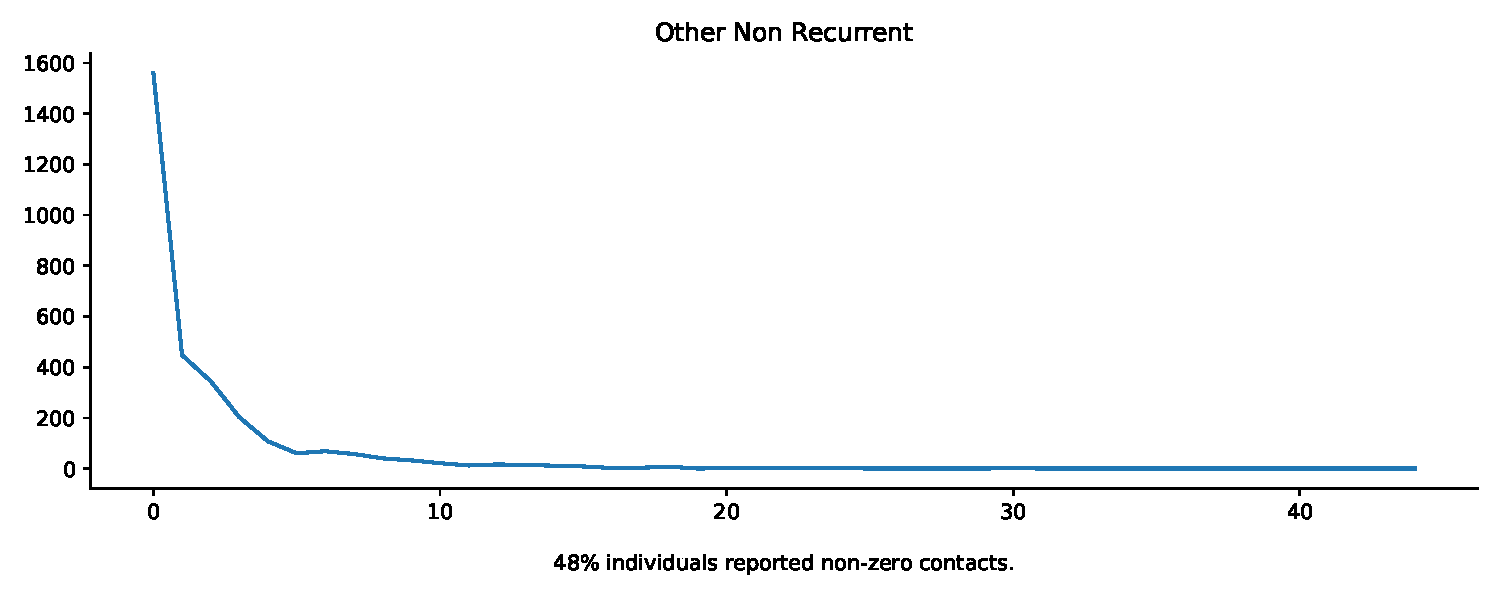
\includegraphics[width=\textwidth]{../figures/results/figures/data/distributions_of_the_number_of_contacts/other_non_recurrent}
    \caption{Number of Non Recurrent Other Contacts}
    \label{n_contacts_other_non_recurrent}
    \floatfoot{\noindent In the model it is sampled every day which of these numbers of
    contacts a person is planned to have. Note that the contact diaries include such high
    values that super spreading events are well possible in our model. The planned number
    of contacts is reduced by policies, seasonality and individual responses to events
    such as receiving a positive rapid test to the number of actual contacts with
    transmission potential. Other contacts include all contacts that are not household
    members, school contacts or work contacts, for example leisure contacts or contacts
    during grocery shopping. We assume that individuals in households with children or
    teachers or retired individuals have additional contacts during school vacations to
    cover things like family visits or travel during vacations. We estimate this to be on
    average 0.5 additional contacts per vacation day.}
\end{figure}


\begin{figure}
    \centering
    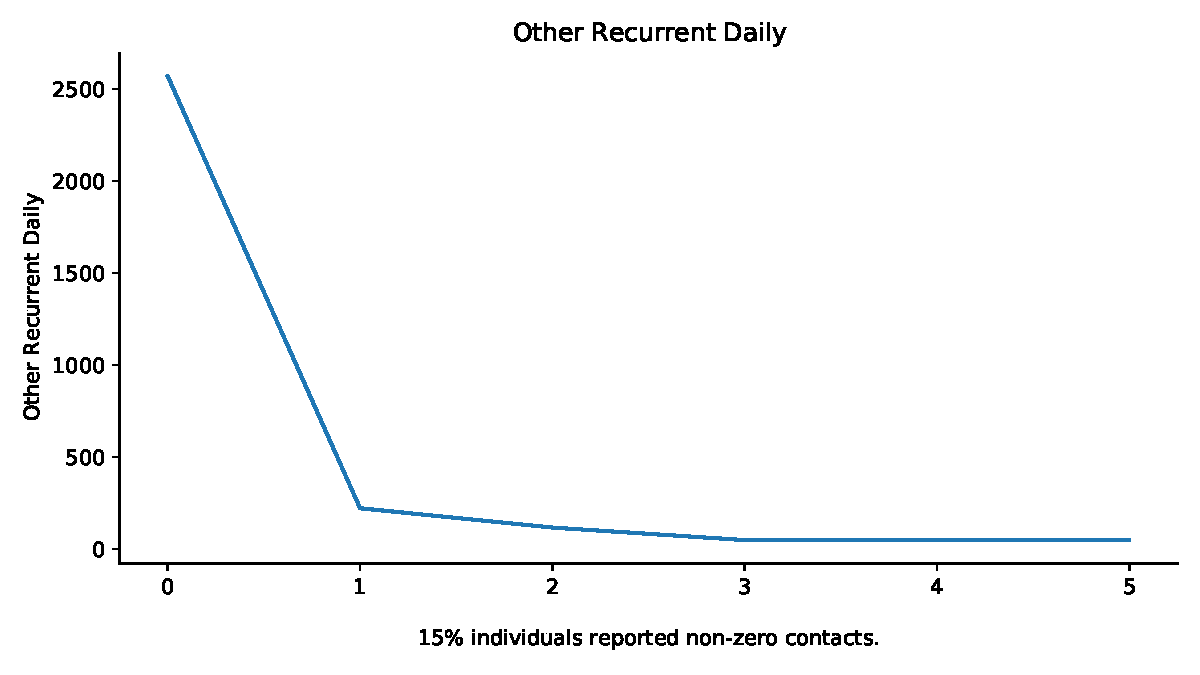
\includegraphics[width=\textwidth]{../figures/results/figures/data/distributions_of_the_number_of_contacts/other_recurrent_daily}
    \caption{Number of Daily Recurrent Other Contacts}
    \label{n_contacts_other_daily_recurrent}
    \floatfoot{\noindent Individuals are assigned to groups that are time constant and
    that meet daily. The share of individuals that attend in a way that has transmission
    potential is reduced by policies, seasonality and individual responses to events such
    as receiving a positive rapid test. Other contacts include all contacts that are not
    household members, school contacts or work contacts, for example leisure contacts or
    contacts during grocery shopping.}
\end{figure}


\begin{figure}
    \centering
    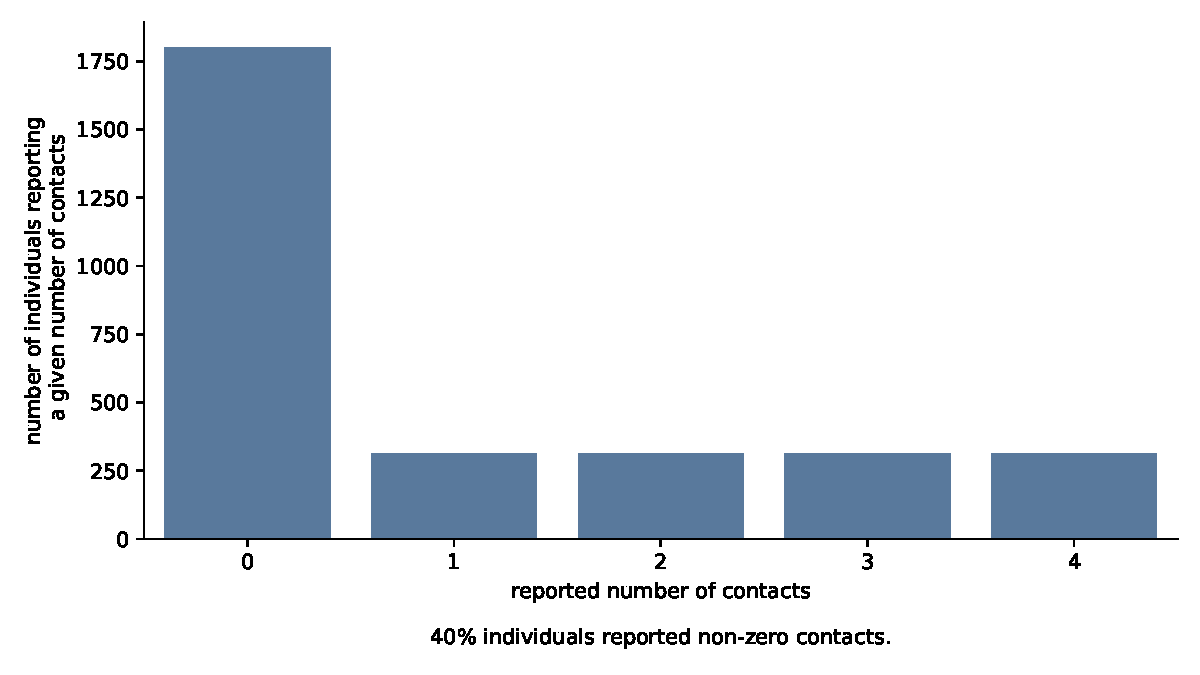
\includegraphics[width=\textwidth]{../figures/results/figures/data/distributions_of_the_number_of_contacts/other_recurrent_weekly}
    \caption{Number of Weekly Recurrent Other Contacts}
    \label{n_contacts_other_weekly_recurrent}
    \floatfoot{\noindent Individuals are assigned to up to four groups that are time
    constant and that meet weekly. The share of individuals that attend in a way that has
    transmission potential is reduced by policies, seasonality and individual responses
    to events such as receiving a positive rapid test. Other contacts include all
    contacts that are not household members, school contacts or work contacts, for
    example leisure contacts or contacts during grocery shopping.}
\end{figure}

% work contacts

\begin{figure}
    \centering
    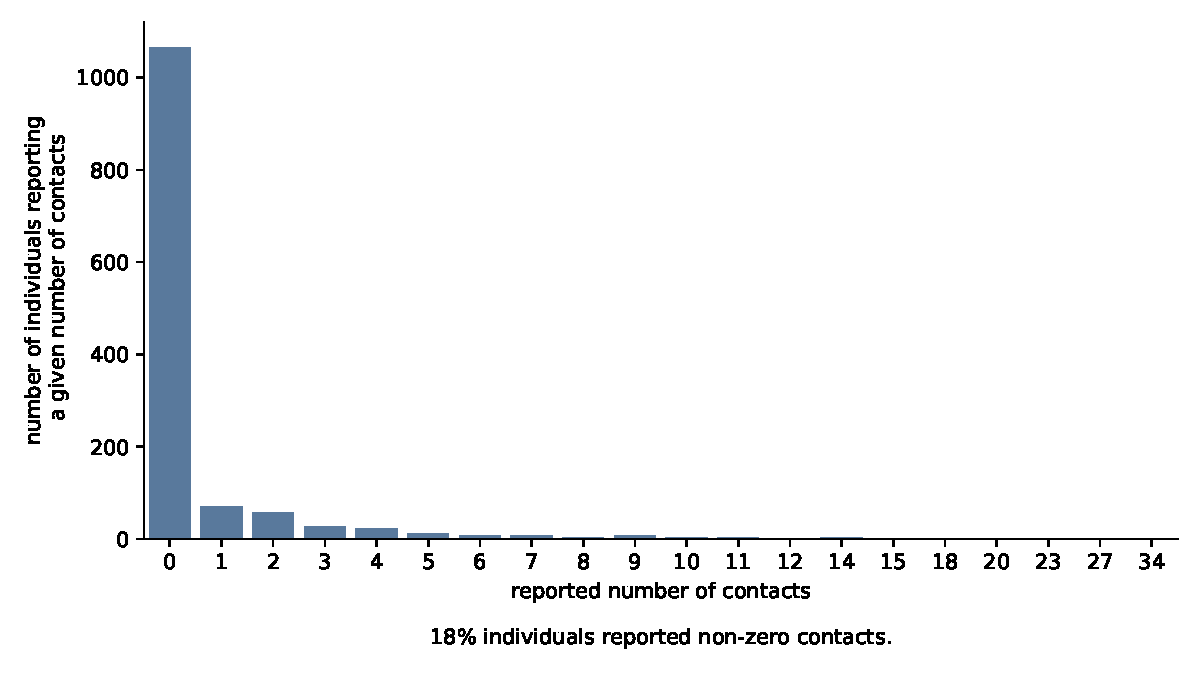
\includegraphics[width=\textwidth]{../figures/results/figures/data/distributions_of_the_number_of_contacts/work_non_recurrent}
    \caption{Number of Non Recurrent Work Contacts}
    \label{n_contacts_work_non_recurrent}
    \floatfoot{\noindent In the model it is sampled every day which of these numbers of
    contacts a working person is planned to have. Note that the contact diaries include
    such high values that super spreading events are well possible in our model. The
    planned number of contacts is reduced by policies, seasonality and individual
    responses to events such as receiving a positive rapid test to the number of actual
    contacts with transmission potential. Work contacts only take place between working
    individuals.}
\end{figure}


\begin{figure}
    \centering
    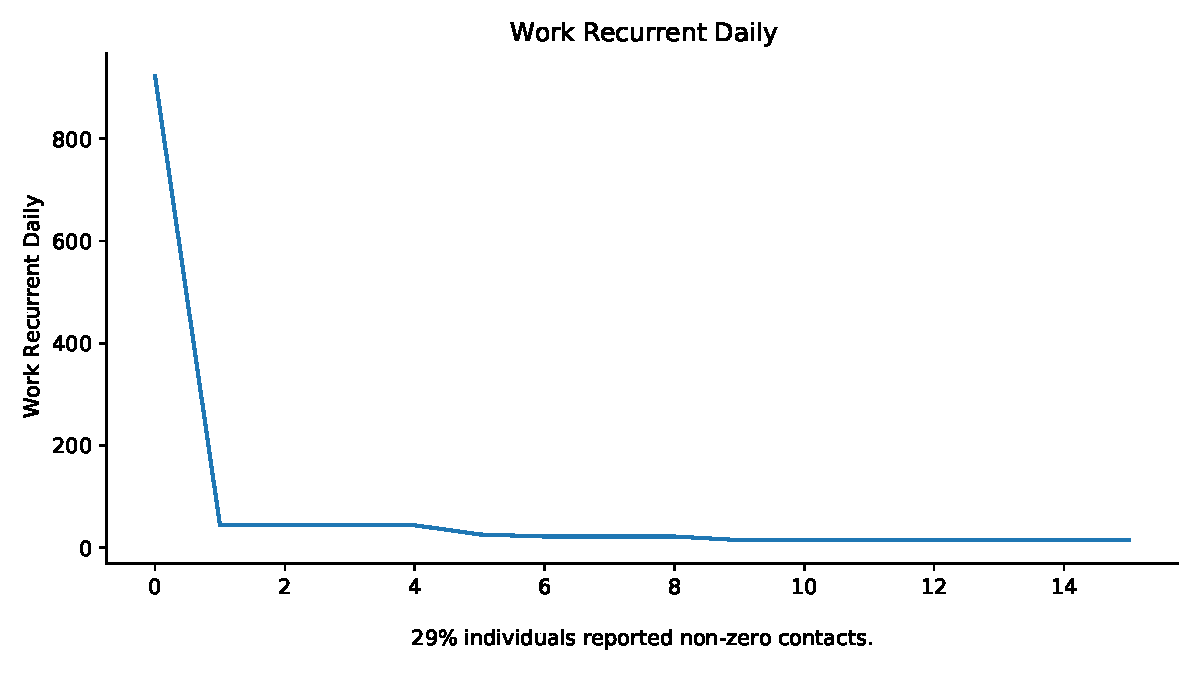
\includegraphics[width=\textwidth]{../figures/results/figures/data/distributions_of_the_number_of_contacts/work_recurrent_daily}
    \caption{Number of Daily Recurrent Work Contacts}
    \label{n_contacts_work_daily_recurrent}
    \floatfoot{\noindent Working individuals are assigned to groups that are time
    constant and that meet daily to match the given distribution of daily work contacts.
    You can think of these as for example colleagues with which one shares an office
    space. The share of individuals that attend in a way that has transmission potential
    is reduced by policies (such as a work from home mandate), seasonality and individual
    responses to events such as receiving a positive rapid test. Work contacts only take
    place between working individuals.}
\end{figure}


\begin{figure}
    \centering
    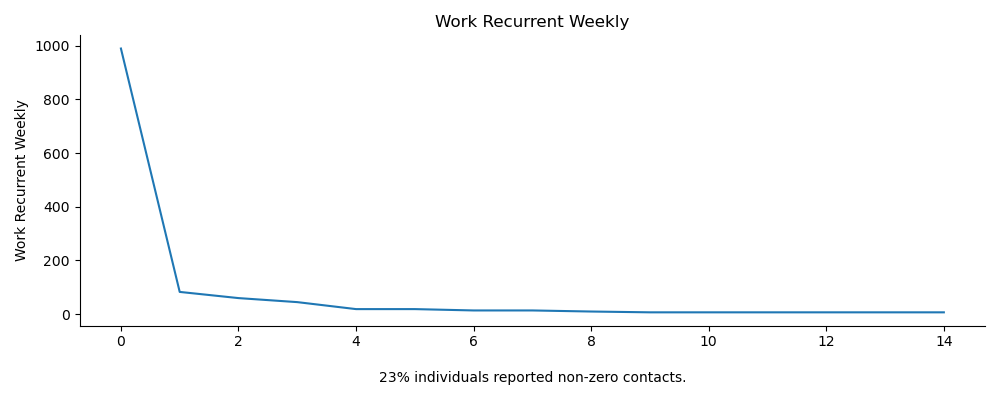
\includegraphics[width=\textwidth]{../figures/results/figures/data/distributions_of_the_number_of_contacts/work_recurrent_weekly}
    \caption{Number of Weekly Recurrent Work Contacts}
    \label{n_contacts_work_weekly_recurrent}
    \floatfoot{\noindent  Working individuals are assigned to up to 14 groups that are time
    constant and meet weekly. Groups are scheduled to meet on separate days of the work
    week. These contact models cover weekly team meetings etc. The share of individuals
    that attend in a way that has transmission potential is reduced by policies,
    seasonality and individual responses to events such as receiving a positive rapid
    test. Work contacts only take place between working individuals.}
\end{figure}


\FloatBarrier


\subsection{Contacts by age}
\label{subsec:contacts_by_age}

As mentioned in section \ref{sec:matching}, the probability that two individuals are
matched can depend on background characteristics. In particular, we allow this
probability to depend on age and county of residence. While we do not have good data on
geographical assortativity and just roughly calibrate it such that 80\% of contacts are
within the same county, we can calibrate the assortative mixing by age from the same
data we use to calibrate the number of contacts.\comment[id=HM]{Redo
\ref{fig:assortativity_other} /\ref{fig:assortativity_work} with total number of
contacts or better add a similar figure showing total number of contacts by age in all
networks}

\begin{figure}[ht]
    \centering
    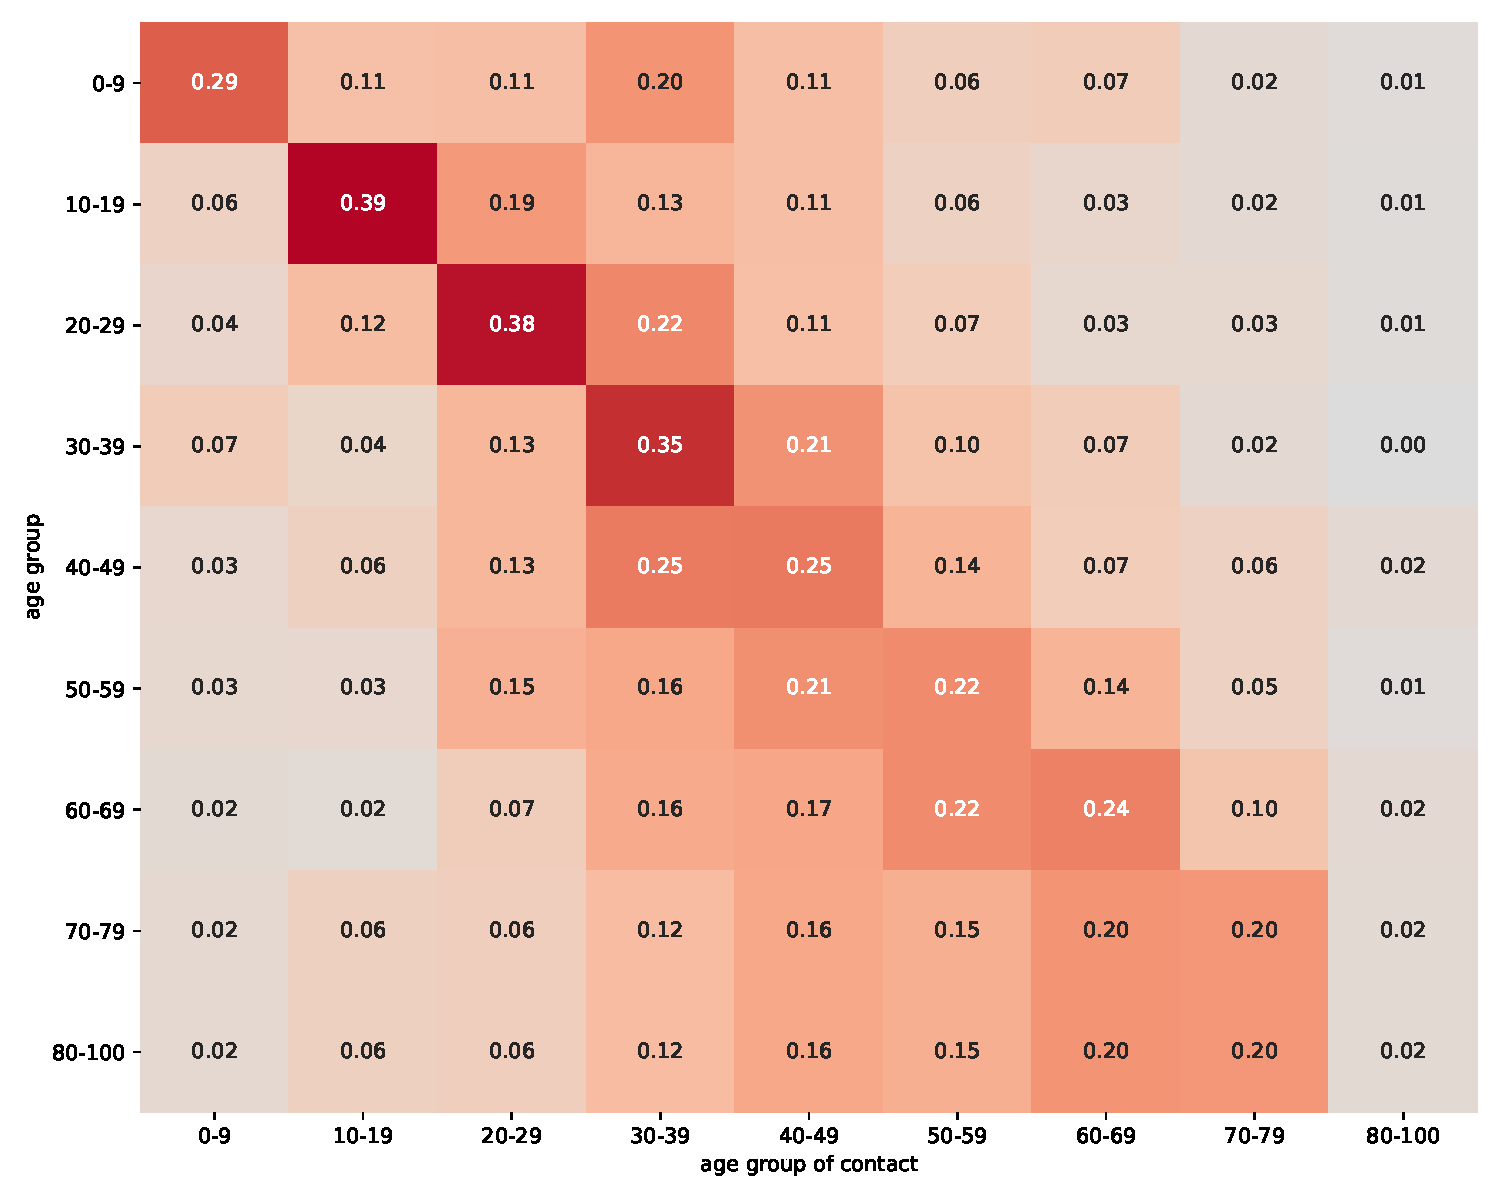
\includegraphics[width=0.9 \textwidth]{../figures/results/figures/data/assortativity_other_non_recurrent}
    \caption{Distribution of Non Recurrent Other Contacts by Age Group}
    \label{fig:assortativity_other}
    \floatfoot{\noindent The figure shows the distribution of non recurrent other contacts by age
        group. A row shows the share of contacts a certain age group has with all other
        age groups. Higher values are colored in darker red tones. The diagonal
        represents the share of contacts with individuals from the same age group.}
\end{figure}


Figure~\ref{fig:assortativity_other} shows that assortativity by age is especially strong
for children and younger adults. For older people, the pattern becomes more dispersed
around their own age group, but within-age-group contacts are still the most common
contacts.

\begin{figure}[ht]
    \centering
    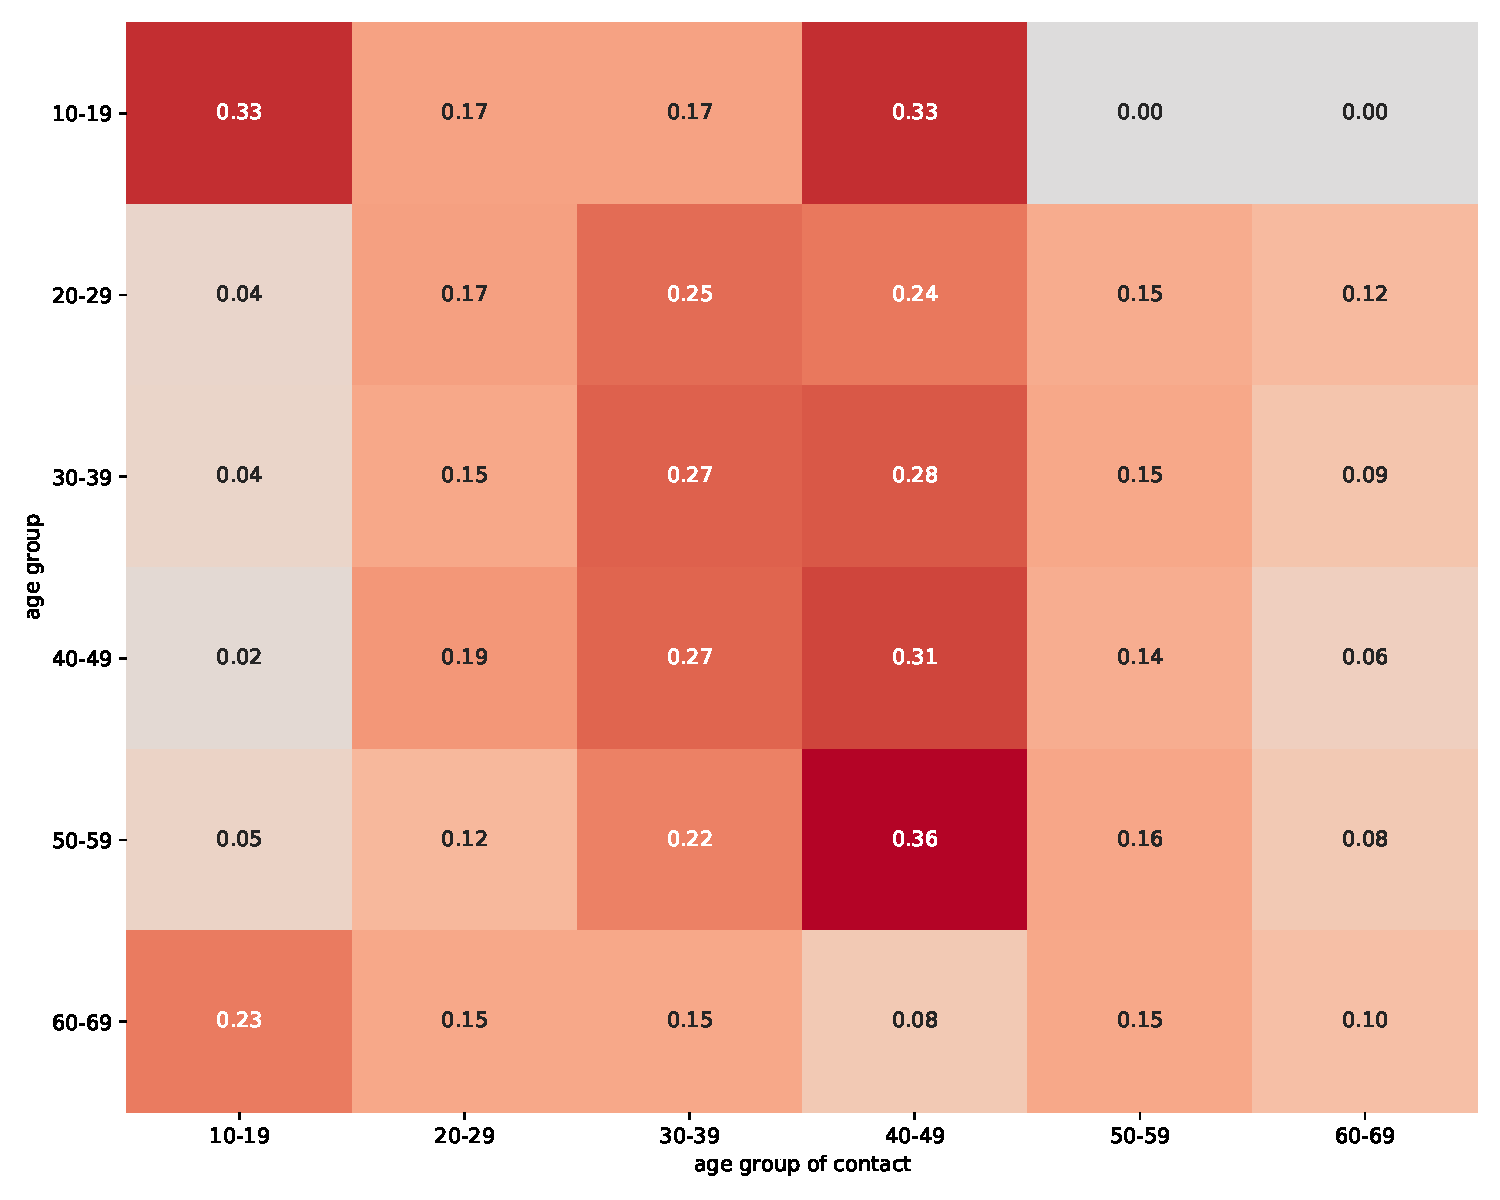
\includegraphics[width=0.9 \textwidth]{../figures/results/figures/data/assortativity_work_non_recurrent}
    \caption{Distribution of Random Work Contacts by Age Group}
    \label{fig:assortativity_work}
    \floatfoot{\noindent The figure shows the distribution of non recurrent work contacts by age
        group. A row shows the share of contacts a certain age group has with all other
        age groups. Higher values are colored in darker red tones. The diagonal
        represents the share of contacts with individuals from the same age group. We
        only show age groups that have a significant fraction of working individuals.}
\end{figure}

Figure~\ref{fig:assortativity_work} shows that assortativity by age is also important
among work contacts.

Our other two types of contacts, households and schools, get their assortativity by
construction. Schools are groups where the same children of the mostly same age group and
county meet with teachers every day. Household composition follows directly from the
German microcensus data we use to construct our synthetic population.\comment[id=HM]{So
no work in here? How about school? Can we add a column with marginals and another one
with work / (school?), too?}\comment[id=K]{I hope adding work and writing about school and
households addresses all questions. I think marginals would be confusing because they may not add up to one given that age groups have different group sizes.}

\FloatBarrier


\subsection{Infection Probabilities}
\label{sec:estimation}

To calibrate infection probabilities outside of the model, it would be important to know
the exact duration and distance of each contact type as well as viral loads. Since this
is not available in any data set, we estimate those parameters inside the model with the
method of simulated moments \citep{McFadden1989} by minimizing the distance between
simulated and observed infection rates. Since our model includes a lot of randomness, we
average simulated infection rates over several model runs.

Currently, we use data for Germany from October 2020 until June 2021. We do not use
earlier periods for three reasons. Firstly, in the beginning PCR tests were highly
limited and therefore it would be difficult to find good initial conditions for our
simulations. In addition during the summer the case numbers were extremely low. This
could lead to the epidemic going extinct in our simulation. Additionally, our model does
not include international travel or other imports of cases. These would be important but
difficult to model during the summer months.

To avoid over-fitting and simplify the numerical optimization problem, we only allow for
five different probabilities: 1) for contacts in schools 2) contacts in preschools and
nurseries. 3) for work contacts. 4) for households. 5) for other contacts.

The infection probabilities estimated from our model are as follows: For household
contacts (each individual meets all his or her household members every day) the infection
probability is 10\%, for school contacts (all students and teachers meet all other
students and teachers that attend school that day and there are three classes taking
place each day) the probability of infection is 1.2\%, for preschools and nurseries that
infection probability is 0.5\%. Work contacts carry a risk of 14.5\% and other activities
(including leisure activities such as meeting friends) carry the highest risk with
15.875\%.

\subsection{Policies}

\FloatBarrier

In our empirical application we distinguish four groups of contact types: households,
education, work and other contacts. For households we assume that the individuals'
contacts in their households do not change over our estimation period. For nurseries,
preschools and schools we implement vacations as announced by the German federal states
as well as school closures, emergency care and A / B schooling where only one half of
students attends every other week or day. For the moment we ignore that lack of childcare
leads working parents to stay home.
%
% Schließung von Kindertagesstätten und Schulen: 37,4 Millionen ausgefallene Arbeitstage
% http://www.iab-forum.de/schul-und-kitaschliessungen-krankheit-quarantaene-die-coronabedingten-arbeitsausfaelle-der-erwerbstaetigen-steigen-auf-592-millionen-arbeitstage/
%
%
% https://www.sueddeutsche.de/politik/schulschliessung-lockdown-bildung-1.5190377: In
% allen Ländern geht trotz des Lockdowns ein erheblicher Anteil der Schülerinnen und
% Schüler in die Schule.
% https://gfx.sueddeutsche.de/apps/e525337/www/_image_desktopw1840q70-1e2e2bf78b7d4430
% 18% der Grundschüler in Notbetreuung in BW
%
For our work models\footnote{We distinguish non-recurrent work contacts, daily work
contacts and weekly work contacts.} we use the reductions in work mobility reported in
the Google Mobility Data \citep{Google2021} to calibrate our work policies. Reductions in
work contacts are not random but governed through a work contact priority where the
policy changes the threshold below which workers stay home. Figure
\ref{fig:work_multiplier} shows the share of workers that go to work in our model over
time.

\begin{figure}[ht]
    \centering
    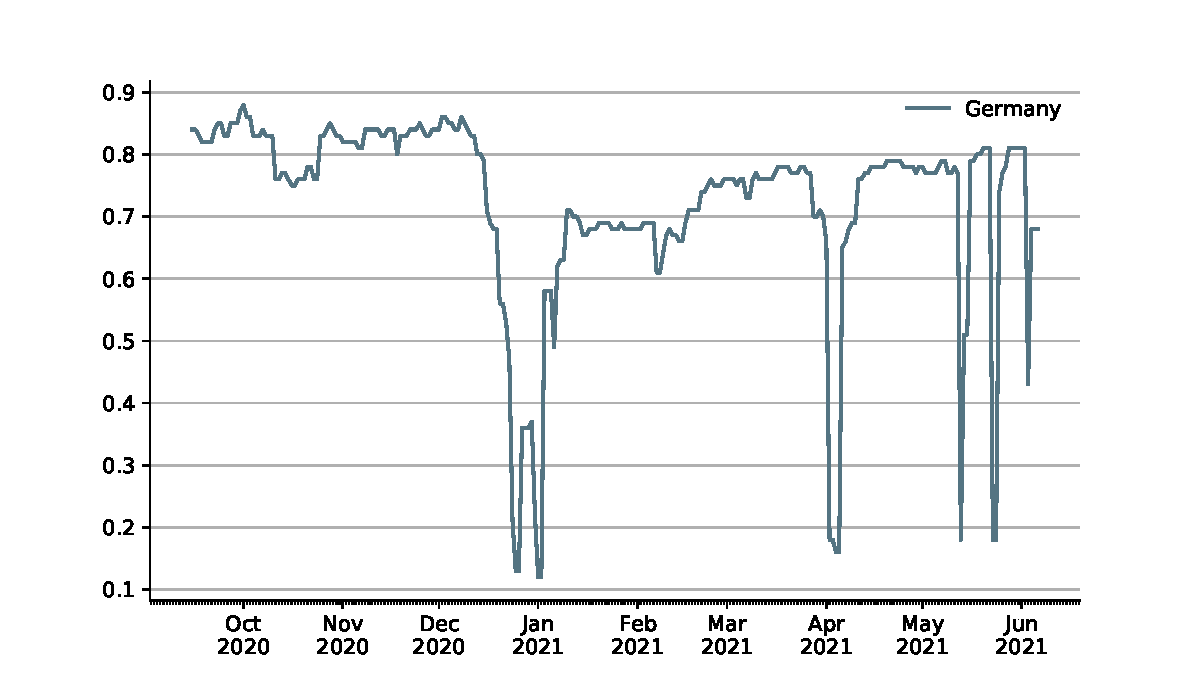
\includegraphics[width=\textwidth]{../figures/results/figures/data/work_multiplier_since_sep}
    \caption{Share of Workers with Work Contacts}
    \label{fig:work_multiplier}
    \floatfoot{\noindent The figure shows the work mobility as reported by \cite{Google2021}. We
        take this as a proxy of the share of workers who are not in home office, i.e. who
        still have physical work contacts. The figure interpolates over weekends as we
        handle weekend effects through information on work on weekends in the German
        census data we use. The figure shows the share aggregated over Germany as a
        whole. To capture the effect that local policies, school vacations and public
        policies have on work contacts we use the data by German state to determine which
        workers go to work depending on the state they live in.}
\end{figure}

For both work and school contacts we assume that starting November with the lockdown
light in Germany, hygiene measures (such as masks, ventilation and hand washing) became
more strict and more conscientiously observed, leading to a reduction of 33\% in the number of contacts with the potential to transmit Covid-19.

For the last group of contacts which cover things like leisure activities, grocery
shopping etc. we have no reliable data by how much policies reduce them. In addition,
they are likely to be affected by social and psychological factors such as pandemic
fatigue and vacations. Because of this we estimate them like the infection probabilities
to fit the time series data. We use very few change points and tie them to particular
events such as policy announcements or particular holidays.\comment[id=K]{@Janos should we already add in numbers in here?}

\FloatBarrier

\subsection{Rapid Test Demand}


\begin{figure}
    \centering
    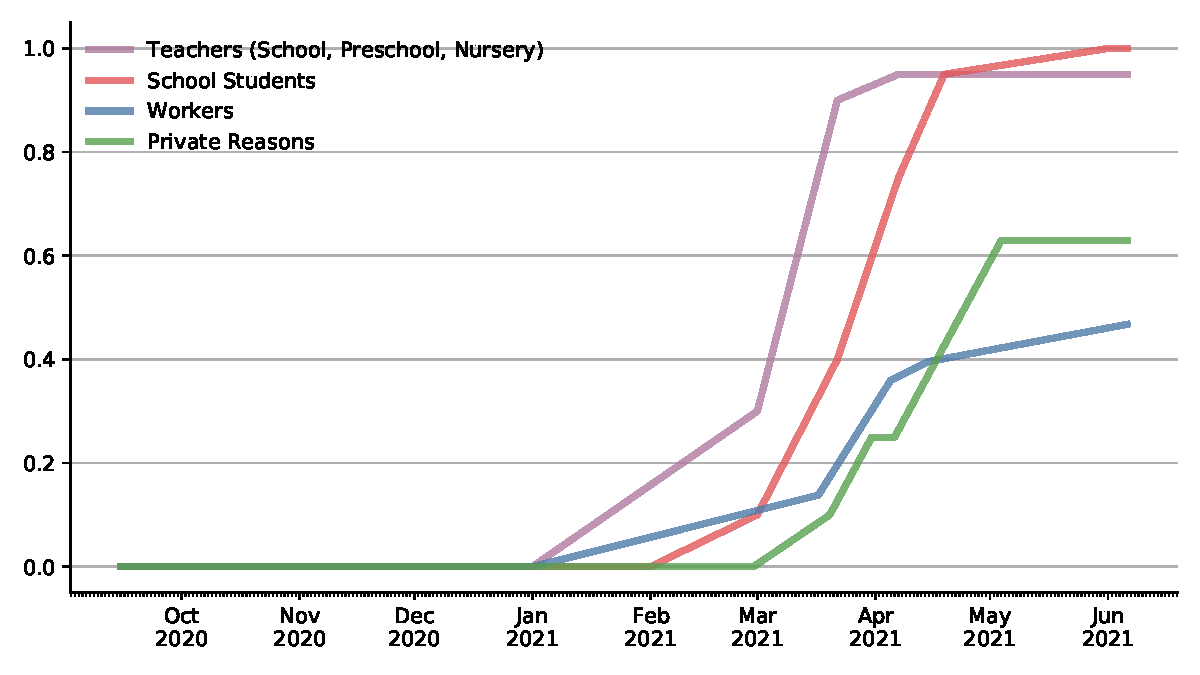
\includegraphics[width=\textwidth]{../figures/results/figures/data/testing/rapid_test_demand_shares}
    \caption{\textbf{Share of Individuals that do a Rapid Test.}}
    \floatfoot{\noindent \textcolor{red}{J: Talk about the interpretation of each line.}}
    \label{fig:rapid_test_demand}
\end{figure}

In our model, there are five reasons why rapid tests are done:
\begin{enumerate}
    \item someone plans to have work contacts
    \item someone is an employees of an educational facility or school pupil
    \item someone lives in a household where someone has tested positive or developed
          symptoms
    \item someone has developed symptoms but has not received a PCR test
    \item someone plans to participate in a weekly non-work meeting
\end{enumerate}

% work rapid tests

For work contacts, we know from the COSMO study (\cite{Betsch2021}, 20th/21st of April)
that 60\% of workers who receive a test offer by their employer regularly use it. We
assume this share to be time constant.

In addition, there are some surveys that allow us to trace the expansion of employers who
offer tests to their employees. Mid march, 20\% of employers offered tests to their
employees \citep{DIHK2021}. In the second half of March, 23\% of employees reported being
offered weekly rapid tests by their employer \citep{Ahlers2021}. This share increased to
60\% until the first days of April \cite{ZDF2021}. Until mid April 70\% of workers were
expected to receive a weekly test offer \citep{AerzteZeitung2021}. However, according to
surveys conducted in mid April \citep{Betsch2021}, less than two thirds of individuals
with work contacts receive a test offer. Starting on April 19th employers were required
by law to provide two weekly tests to their employees \citep{Bundesanzeiger2021}. We
assume that compliance is incomplete and only 80\% of employers actually offer
tests.\comment[id=HM]{Can we use the IZA/BMAS survey? Not sur about citing evening news
in scientific papers.}\comment[id=K]{I am not aware of any survey looking at compliance.
If you know of some, that would be great. Updating this might change our results but it
would definitely be an improvement!}

% educ rapid tests

We assume that employees in educational facilities start getting tested in 2021 and that
by March 1st 30\% of them are tested weekly.

The share increases to 90\% for the week before Easter. At that time both Bavaria
\citep{BayrischerRundfunk2021} and Baden-Württemberg \citep{MinisteriumKultus2021} were
offering tests to teachers and North-Rhine Westphalia \cite{DPA2021} and Lower Saxony
\citep{SueddeutscheZeitung2021} were already testing students and tests for students and
teachers were already mandatory in Saxony \citep{SueddeutscheZeitung2021a}. After Easter
we assume that 95\% of teachers get tested twice per week.\comment[id=K]{Mostly newspaper
articles and one KuMi press communication. I have more sources for the smaller federal
states but they are extremely time consuming to enter into the references.}


% --------------------------------------------------------------------------------------
%
%def _add_educ_rapid_test_fade_in_params(params):
%    """Add the shares how many people with educ contacts get a rapid test.
%
%    Sources:
%        - 17-24 of March 2021 (Mon, 2021-03-22):
%            - NRW had 80% tests for students before Easter (https://bit.ly/3u7z8Rx)
%            - BY: test offers to educ_workers (https://bit.ly/3tbVX5u)
%            - BW: only tests for educ workers (https://bit.ly/2S7251M)
%
%            - federal level:
%                "In Kitas und Schulen sollen die Testmöglichkeiten "mit der
%                steigenden Verfügbarkeit von Schnell- und Selbsttests"
%                ausgebaut werden" (https://bit.ly/3nuCSKi)
%            - Some KiTa workers are being tested (https://bit.ly/3nyGyus)
%            - Self tests for students in Berlin (https://bit.ly/2ScGu8m)
%            - Schleswig-Holstein: test offer (https://bit.ly/3eVfkuv)
%            - mandatory tests in Saxony (https://bit.ly/3eEQGhn)
%            - no tests yet for students in Hessia, but already ordered
%              (https://bit.ly/3gMGJB4)
%            - Niedersachsen had one test week before Easter (https://bit.ly/3gOOC96)
%
%            => assume 90% of teachers and 40% of students do rapid tests
%
%        - After Easter (2021-04-07):
%            - NRW: tests are mandatory for all
%            - Bavaria: tests are mandatory for all (https://bit.ly/3nz5fXS,
%              https://bit.ly/2QHilX3)
%            - BW: voluntary tests for students (https://bit.ly/3vuetaD)
%            - Brandenburg starts with tests (https://bit.ly/3xAihZB)
%            - Schleswig-Holstein: mandatory tests (https://bit.ly/3eVfkuv)
%
%            => assume 95% of teachers and 75% of students get tested
%
%        - BW: tests mandatory starting 2021-04-19 (https://bit.ly/3vuetaD)
%
%            => assume 95% of teachers and 95% of students get tested
%
%    """
%    params = params.copy(deep=True)
%
%    loc = ("rapid_test_demand", "educ_worker_shares")
%    params.loc[(*loc, "2020-01-01"), "value"] = 0.0
%    params.loc[(*loc, "2021-01-01"), "value"] = 0.0
%    # this is arbitrary to have a more convex shape
%    params.loc[(*loc, "2021-03-01"), "value"] = 0.3
%    params.loc[(*loc, "2021-03-22"), "value"] = 0.9
%    params.loc[(*loc, "2021-04-07"), "value"] = 0.95
%    params.loc[(*loc, "2021-04-19"), "value"] = 0.95
%    params.loc[(*loc, "2021-06-01"), "value"] = 0.95
%    params.loc[(*loc, "2025-12-31"), "value"] = 0.95
%
%    loc = ("rapid_test_demand", "student_shares")
%    params.loc[(*loc, "2020-01-01"), "value"] = 0.0
%    params.loc[(*loc, "2021-02-01"), "value"] = 0.0
%    params.loc[(*loc, "2021-03-01"), "value"] = 0.1
%    params.loc[(*loc, "2021-03-22"), "value"] = 0.4
%    params.loc[(*loc, "2021-04-07"), "value"] = 0.75
%    params.loc[(*loc, "2021-04-19"), "value"] = 0.95
%    params.loc[(*loc, "2021-06-01"), "value"] = 1.0
%    params.loc[(*loc, "2025-12-31"), "value"] = 1.0
%
%    # Assume weekly tests before Easter and twice weekly tests after Easter
%    # We should get a fade-in through different ends of Easter vaccation
%    params.loc[("rapid_test_demand", "educ_frequency", "before_easter"), "value"] = 7
%    params.loc[("rapid_test_demand", "educ_frequency", "after_easter"), "value"] = 3
%
%    return params
%
% --------------------------------------------------------------------------------------


\comment[id=J]{Sources still missing below this}

Tests for students started later so we assume that they only start in February and only
10\% of students get tested by March 1st. Relying on the same sources as above we
approximate that by the week before Easter this share had increased to 40\%.

After Easter we assume the share of students receiving twice weekly tests to based on
tests already being mandatory in North-Rhine Westphalia and Bavaria while still being
voluntary in Baden-Württemberg. There tests become mandatory on April 19th.


% household member rapid tests



% own symptom rapid test demand



% private meeting test demand



\comment[id=J]{Add a section on how we calibrate rapid test demand; Mainly describe the
datapoints we have and say that we usually interpolate linearly in between data points.
(Only exception to that is private rapid test demand, which we fit to data)}


\begin{figure}[ht]
    \centering
    \caption{Share of Individuals With Rapid Tests}
    \label{fig:share_ever_rapid_test}
    \begin{subfigure}{.55\textwidth}
        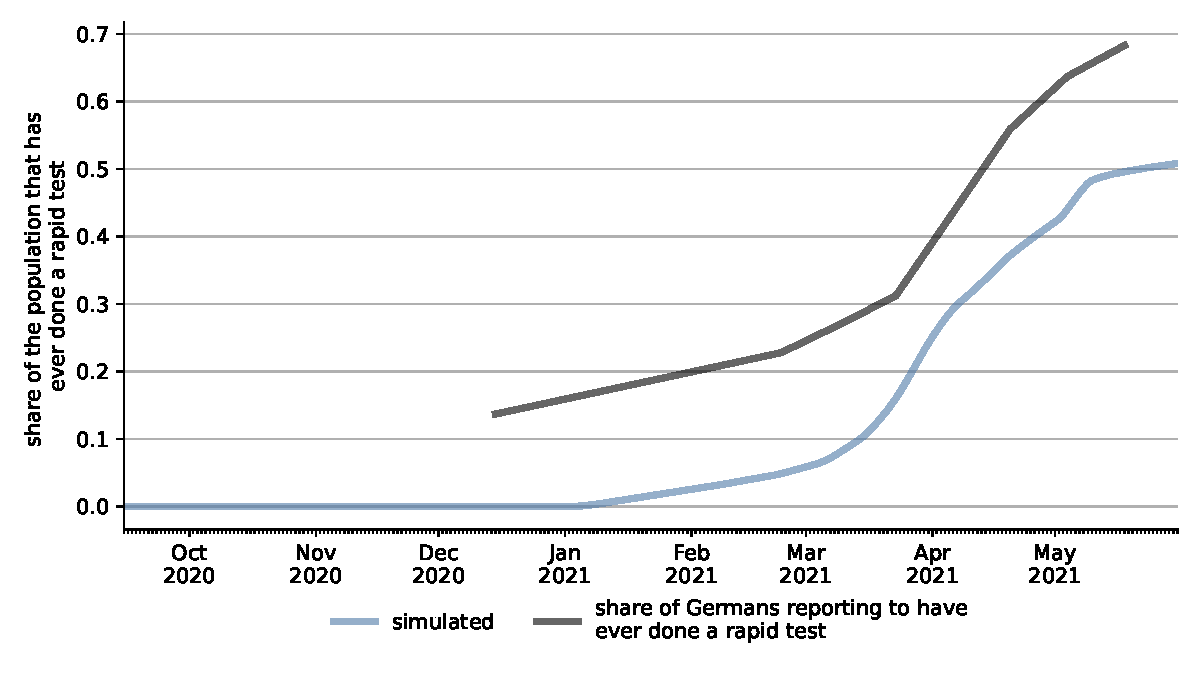
\includegraphics[width=0.9 \textwidth]{../figures/results/figures/scenario_comparisons/combined_fit/full_share_ever_rapid_test}
    \end{subfigure}%
    \begin{subfigure}{.55\textwidth}
        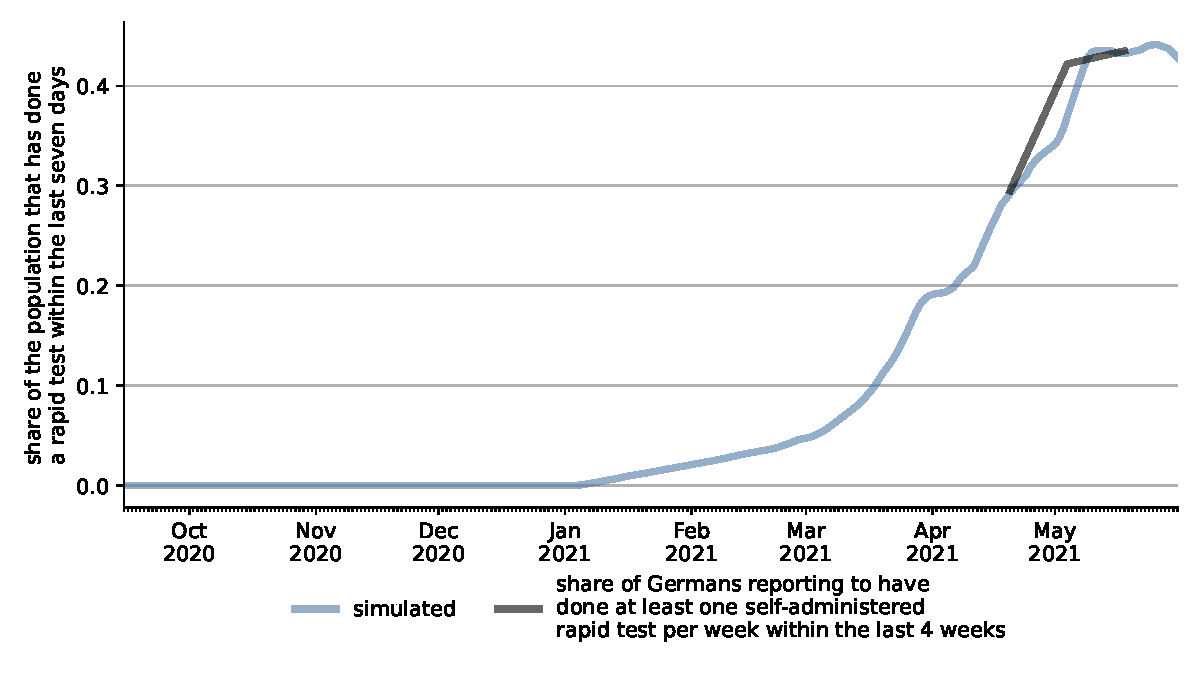
\includegraphics[width=0.9 \textwidth]{../figures/results/figures/scenario_comparisons/combined_fit/full_share_rapid_test_in_last_week}
        %   \caption{Share of Individuals Having Done a Rapid Test in the Last Week}
    \end{subfigure}
    \label{fig:share_rapid_test_last_week}
    \floatfoot{\noindent The figure compares the share of individuals who have ever done a rapid
        test or done a rapid test within the last week in our simulations to the shares
        reported in the
        \href{https://projekte.uni-erfurt.de/cosmo2020/web/topic/wissen-verhalten/80-schnelltests/}{COVID-19
            Snapshot Monitoring survey}. The left panel compares the share of individuals
        who have ever done a rapid test. The right panel compares the share of
        individuals who have done a rapid test within the last seven days in our
        simulation compared to the share reporting to have done at least weekly rapid
        tests in the last four weeks in the COSMO survey. Overall our calibration of
        rapid tests are slightly conservative. The overall share is below that in the
        study. We fit the share of weekly tests quite exactly. However, the study only
        covers adults while our share also includes children who are tested very
        regularly when attending school.}
\end{figure}
